\section{Analysis overview}
\label{sec:analysis_overview}

%Many diboson analyses are being performed with Run 2 2016 data by CMS collaboration, covering a plethora of different final states. In this thesis, a search for diboson resonances in the $\nu \bar{\nu} q \bar{q}$ is performed. 
This analysis searches for potential signals of heavy resonances decaying into a pair of vector bosons, using the data collected by the CMS experiment during 2016, corresponding to an integrated luminosity of $\mathcal{L}=35.9 \mbox{ fb}^{-1}$. One of the boson should be a \Z, and it is identified through its invisible decay into a couple of neutrinos ($\nu \bar{\nu}$), while the other electroweak boson, labelled as \V and consisting either in a \W or in a \Z boson, is required to decay hadronically into a pair of quarks ($q \bar{q}$). %The final states probed by this analysis therefore consists in two quarks and two neutrinos, reconstructed as missing transverse energy (\met).
The decay products (the bosons) of heavy (around the TeV scale) resonances are produced with large Lorentz boosts; as a consequence, the decay products of the bosons (quarks and neutrinos) are expected to be highly energetic and collimated. In this regime, the standard jet reconstruction algorithms fail in distinguishing the two jets from the quarks, suggesting to look for a signature composed of a large-cone high-\pt jet, in which both $q$ and $\bar{q}$ lie, recoiling against a large amount of missing transverse momentum (\met) due to the neutrinos escaping the detector. The hadronically decaying boson ($Z$, $W$) is then reconstructed as one large-cone jet, whose mass is used to define the signal region and signal-depleted control regions, the sidebands. %Jet substructure techniques are exploited in order to suppress background contamination and to classify the events in two exclusive signal purity categories, allowing to improve the discovery reach.
The analysis of the jet substructure improves the background suppression and it allows to group the events in two mutually exclusive categories, with different signal purity, enhancing the sensitivity of the search.

\noindent A general $ZZ$ decay, predicted by the bulk graviton model (sec.~\ref{sec:BG}), can be reconstructed both in final states with high signal purity but limited statistics (four charged leptons) and large statistics but overwhelming backgrounds (no charged leptons). The choice to look for one boson decaying hadronically and the other $Z$ into neutrinos represents the best compromise between these two extremes. This topology can be also utilized to reconstruct a charged spin-1 vector boson \Wp decaying into an invisible $Z$ and an hadronic $W$, predicted by the HVT model (sec.~\ref{sec:theory_HVT}), making this analysis sensitive to a generic \VZ final state.

\noindent Signal events are collected with trigger paths requiring high \met recoiling against jet activity. This signature is clearly a very challenging one in an environment with more than 50 primary collisions per bunch crossing. For this reason, the Particle-Flow algorithm is run at trigger level to obtain the highest possible resolution on the jets and thus on the \met.

\noindent The search is performed by examining the distribution of the diboson reconstructed transverse mass of the resonance \VZ (\mtVZ) for a localized excess. The shape and normalization of the main background of the analysis (namely, the production of an electroweak boson in association with jets) are estimated with a data-simulation hybrid approach using the distribution of data in the sidebands, corrected for a function accounting for potential differences between the signal region and the sidebands. The predictions of the secondary background sources completely rely on simulations.

\noindent In fig.~\ref{fig:event_display}, a typical signal event of the \Wpinv process, reproduced with a realistic simulation of the CMS detector, is displayed; the mass of the \Wp is 2.5 TeV. The muon chambers in the barrel (DTs, in light red) and in the endcaps (CSCs, in light blue), along with the tracker detector (green) are shown in the $(r, \varphi)$ transverse plane (left) and the $(r, z)$ longitudinal plane (right). The large-cone jet, identifying the \W hadronic decay, is displayed in red; the energy deposits in ECAL (light orange) and in HCAL (in violet) can be seen in the pictures. The missing transverse energy, signature of the \Z invisible decay, is represented as a blue arrow, lying in the transverse plane. %The track multiplicity (green tracks) is shown in the center of the detector, where the tracker is installed.
Green tracks represent charged particles from the underlying events as reconstructed by the silicon tracker.

\begin{figure}[!htb]
  \centering
    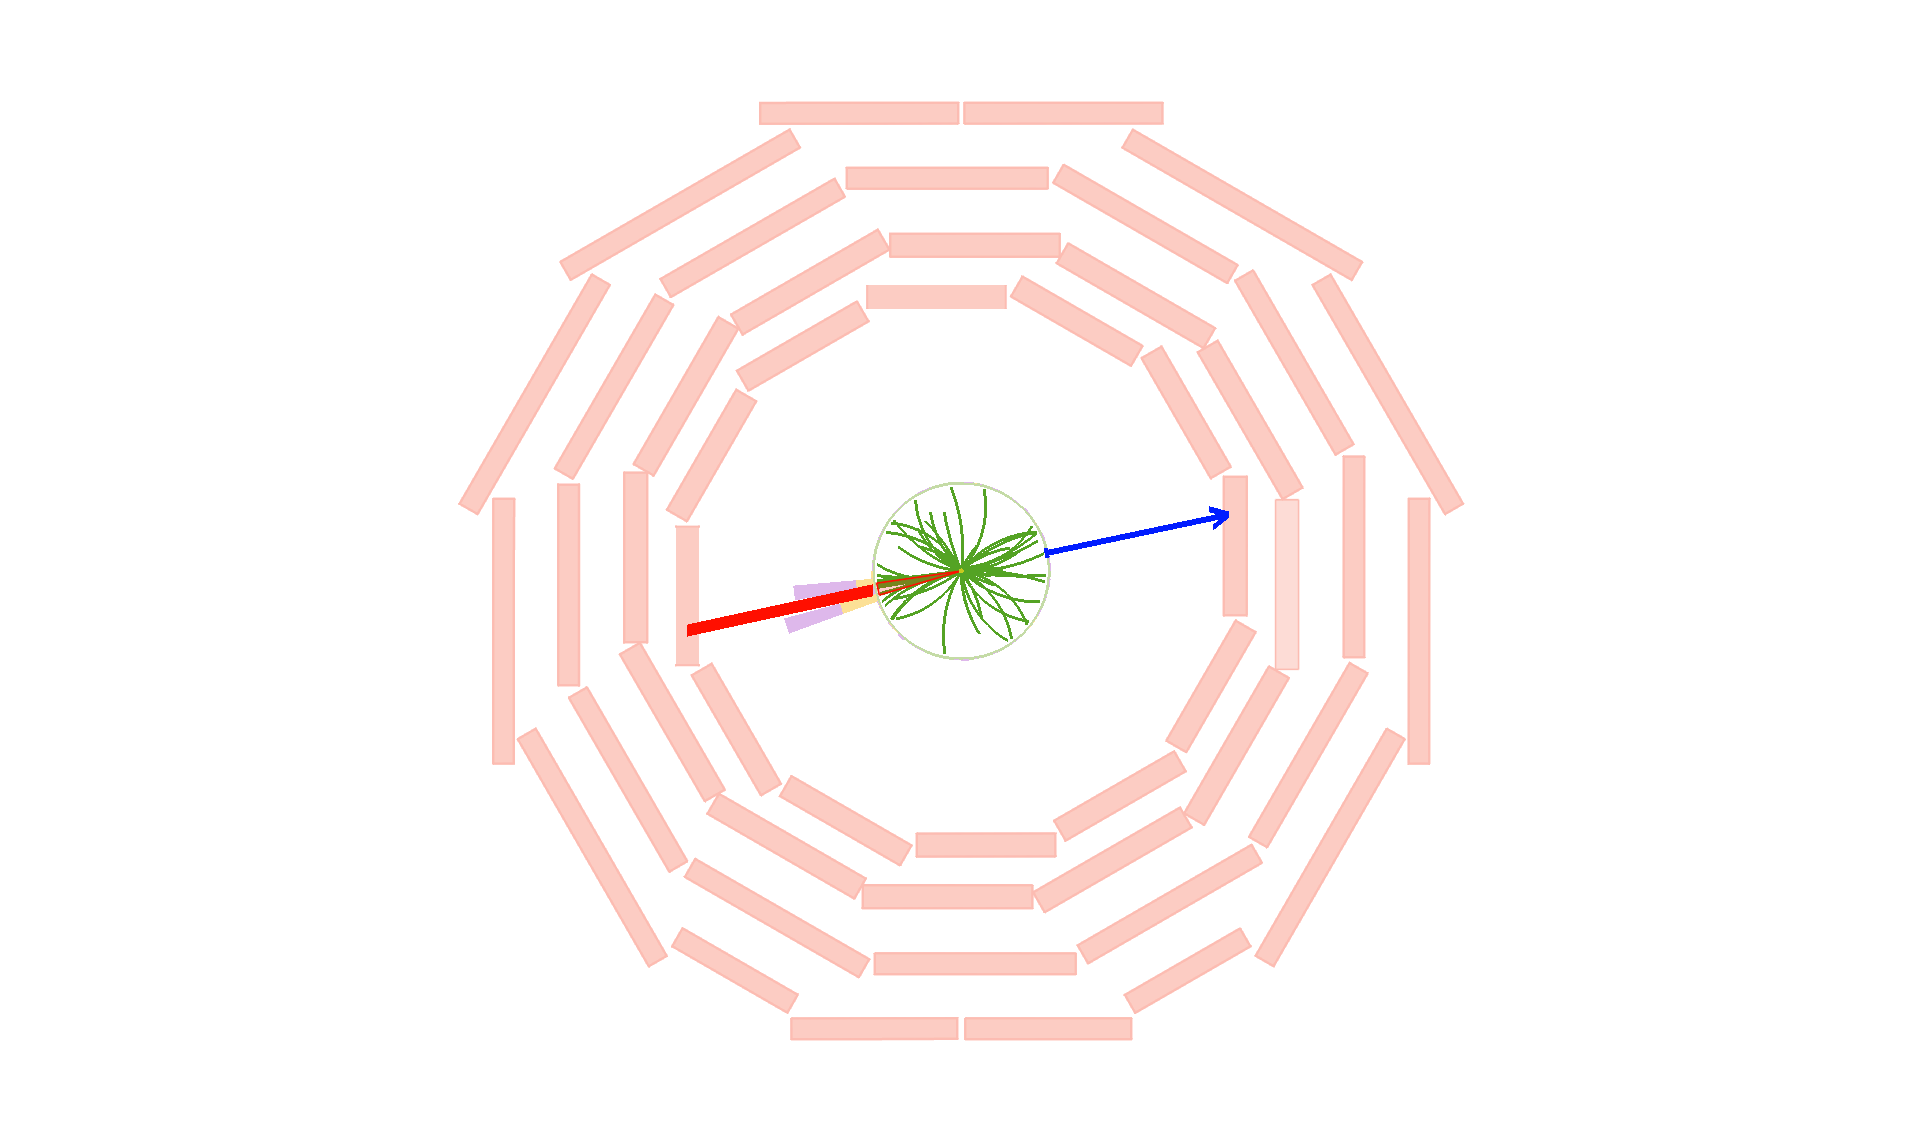
\includegraphics[width=.5\textwidth]{evdisp/Wprime25Tev_rhophi_all.png}%
    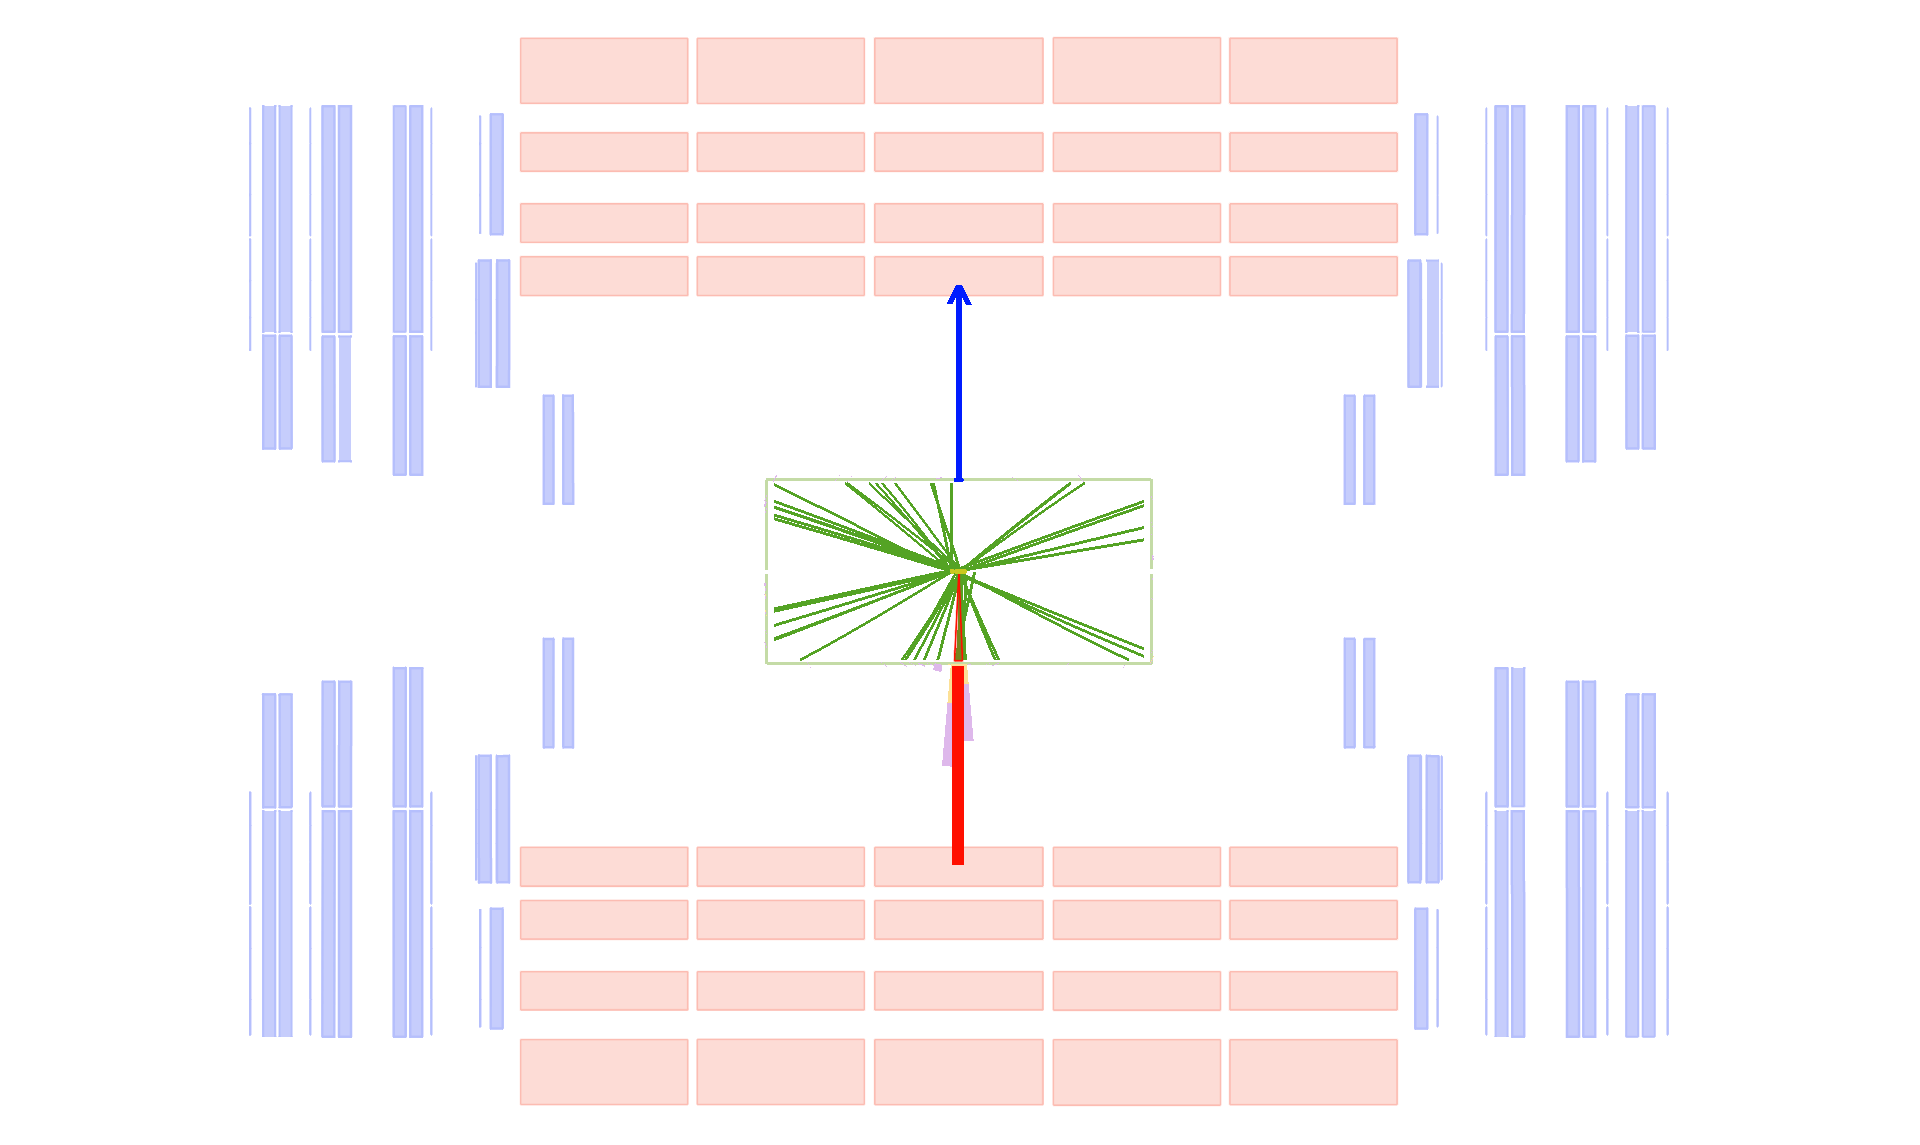
\includegraphics[width=.5\textwidth]{evdisp/Wprime25Tev_rhoz_all.png}%

  \caption{Left: representation of the decay of a \Wp of mass 2.5 TeV, in the transverse plane of the CMS detector. Right: representation of the same event, in the longitudinal plane of the CMS detector.}
  \label{fig:event_display}
\end{figure}
